\documentclass[a4paper,portrait]{scrartcl}

\usepackage[utf8]{inputenc}
\usepackage[T1]{fontenc}
\usepackage{lmodern}
\usepackage[german]{babel}
\usepackage{amsmath}
\usepackage{amssymb}
\usepackage{pst-tree}
\usepackage{graphicx}
\usepackage{tikz}
\usetikzlibrary{positioning,automata}
\usepackage{fancybox}
\usepackage{color}
\usepackage{hyperref}
\hypersetup{allcolors=black}
\title{GBI Zusammenfassung}
\author{Jessica Ochs und Andreas Mai}
\date{17.02.2016}
\begin{document}

\maketitle
\begin{center}
\textbf{GBI Klausur am 02.03.2016} \\
\textbf{14:00 - 16:00} 
\end{center}

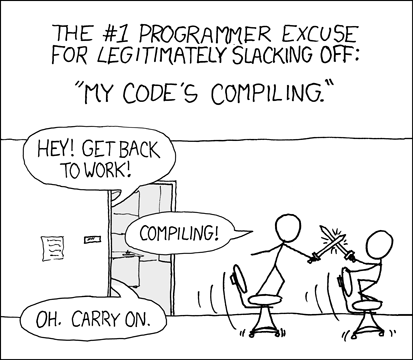
\includegraphics{compiling}
\begin{center}
\textit{Kein Anspruch auf Vollständigkeit ;)}
\end{center}\clearpage
\tableofcontents
\clearpage
\setcounter{page}{1}

\section{Mengen}
\subsection{Kartesisches Produkt}
\begin{itemize}
\item $ M \times N = \lbrace (m,n)\mid m \in M, n \in N \rbrace $
\item $ A \times \varnothing = \varnothing  $
\end{itemize}
\section{Relationen}
\subsection{Funktionen}
\begin{itemize}
\item Funktion = Rechtseindeutige und Linkstotale Relation
\item Injektive Funktion = Linkseindeutige Funktion
\item Surjektive Funktion = Rechtstotale Funktion
\item Bijektive Funktion = Injektive und Surjektive Funktion 
\end{itemize}
\subsection{Potenzmengen}
\begin{itemize}
\item $ \mathcal{P} (M) $ ist die Menge aller möglichen Teilmengen von $M$ 
\item $ \forall M_{i} \subseteq M: M_{i} \in \mathcal{P} (M) $
\end{itemize}
\subsection{Mengengleichheit}
\begin{itemize}
\item $ A=B \Leftrightarrow A \subseteq B \wedge B \subseteq A $ 
\item $ A \setminus B \Leftrightarrow \lbrace x \in A \wedge x \notin B \rbrace $
\end{itemize}
\section{Wörter}
\begin{itemize}
\item Alphabet = Endliche Menge von Zeichen 
\item Wort $w$ aus dem Alphabet $A$ ist eine Folge von konkatenierten Zeichen aus $A$ 
\item $A^{*}$ = Menge aller Wörter über $A$
\end{itemize}
\subsection{Konkatenation}
\begin{itemize}
\item $w_{1} \circ w_{2} \neq w_{2} \circ w_{1}$ 
\item $w = w_{1} \circ w_{2} $ und $ w_{1} \in A^{*}, w_{2} \in B^{*} \Rightarrow w \in (A \cup B)^{*}$
\end{itemize}
\subsection{Das Leere Wort}
\begin{itemize}
\item $ \varepsilon := P_{0} \rightarrow A $ 
\item $ \varepsilon : \lbrace\rbrace\rightarrow\lbrace\rbrace $
\end{itemize}
\subsection{Länge eines Wortes}
\begin{itemize}
\item $ |w^{k}| = k * |w|  $ 
\item $ |\varepsilon| = 0 $ 
\item $ |a \circ b|=|a|+|b| $ 
\item $A^{n}$ ist die Menge aller Wörter der Länge $n$ 
\item $A^{*} = \bigcup\limits_{i = 0}^{\infty} A^{i}$
\end{itemize}
\section{Binäre Operationen}
\begin{itemize}
\item Eine Binäre Operation auf einer Menge M ist eine Abbildung $\diamond: M \times M \rightarrow M$ 
\item kommutativ: $ \forall x,y \in M: x \diamond y = y \diamond x $ 
\item assoziativ: $ \forall x,y,z \in M: (x \diamond y) \diamond z = x \diamond (y \diamond z)$\\
\end{itemize}
\section{Aussagenlogik}
\begin{itemize}
\item $ Var_{AL} $ = Menge aller Aussagevariablen \\
Beispiel: $ Var_{AL} = \lbrace A,B,C \rbrace$
\item $ For_{AL} $ = Menge aller möglichen Formeln über $ Var_{AL} $ \\
Beispiel: $ For_{AL} = \lbrace A \rightarrow B, ...\rbrace$
\end{itemize}
\section{Induktion}
\begin{itemize}
\item Behauptung
\item Induktionsanfang: Zeige: Behauptung gilt für $ n = 0 $
\item Induktionsvoraussetzung: Die Beh. gelte für ein beliebiges aber festes $n \in \mathbb{N}_{0}$
\item Induktionsschritt: Zeige: Behauptung gilt für $ n + 1 $
\end{itemize}
\section{Formale Sprachen}
Sei $A$ ein Alphabet. Die Formale Sprache $ L \subseteq A^{*}$ ist eine Sprache, die alle laut $L$ syntaktisch korrekten Gebilde enthält
\subsection{Produkt formaler Sprachen}
$ L_{1} * L_{2} = \lbrace w_{1}*w_{2} \mid w_{1} \in L_{1} \wedge w_{2} \in L_{2} \rbrace $
\subsection{Potenz Formaler Sprachen}
$ L^{0} = \lbrace \varepsilon \rbrace $ \\
$ L^{i+1} = L^{i}*L$ $(i \in \mathbb{N}_{0})$
\subsection{Konkatenationsabschluss}
$L^{*} = \bigcup\limits_{i = 0}^{\infty} L^{i}$
\subsubsection{$\varepsilon$ -freier Konkatenationsabschluss:}
$L^{+} = \bigcup\limits_{i = 1}^{\infty} L^{i}$ \\
Achtung: Allgemein gilt nicht $ \varepsilon \notin L^{+} $
\section{Übersetzung von Wörtern in Zahlen}
Ich will ja nicht klugscheißen, aber meinst du nicht Codierung?? \\
\begin{itemize}
\item Zahlenbasis $b$
\item $ Num_{b}(\varepsilon) = 0 $ 
\item $ \forall w \in \mathbb{Z}_{0}^{*}, \forall x \in  \mathbb{Z}_{0}: Num_{b}(w * x) = b*Num_{b}(w) + num_{b}(x)$ 
\item $ Num_{b} $ ist die Umrechnung aus dem Binärsystem in das Dezimalsystem 
\item $ Repr_{k}(n) $ ist das kürzesze Wort $ w \in \mathbb{Z}_{k}^{*} $ mit $ Num_{k}(w) = n $, \\also $ Num_{k}(Repr_{k}(n)) = n $\\
Achtung: Im allgemeinen: $Repr_{k}(Num_{k}(w)) \neq w$ 

\item \begin{tabular}{p{1cm}l}
$ Repr_{k}: $&$ \mathbb{N}_{0} \rightarrow \mathbb{Z}_{k}$\\

& $ n\mapsto\begin{cases}
repr_{k}(n)&\text{wenn } n<k \\
Repr_{k}(n\:div\:k)*repr_{k}(n\:mod\:k)&\text{wenn } n \geq k
\end{cases}$
\end{tabular}
\end{itemize}
\subsection{Zweierkomplement}
\begin{itemize}
\item Bietet die Möglichkeit, negative Zahlen Binär darzustellen
\item Vorteilhaft bei Berechnungen im Prozessor
\item $Zkpl_{k}(x) = \begin{cases}
0 * bin_{k-1}(n)&\text{wenn } x\geq 0 \\
1 * bin_{k-1}(2^{k1}+x)&\text{wenn } x<0
\end{cases}$
\end{itemize}
\section{Homomorphismus}
\begin{itemize}
\item Strukturerhaltene Abbildung
\item Kann Präfixfrei und $\varepsilon$-frei sein
\end{itemize}
\subsection{Strukturerhaltend}
$ \forall x,y \in A^{*}: A(xy) = h(x)\circ h(y) $ \\
Beispiel: $h(a) = 2, h(b) = 3 \Rightarrow h(aba) = 232$ 
\subsection{$\varepsilon$-frei}
$ \forall x \in A: h(x) \neq \varepsilon $ \\
Beispiel: $ Kann ich nicht lesen $
\subsection{Präfixfrei}
$ \forall x \in A^{*}\: \nexists \:v,z \in A^{*} \wedge w \neq vz: h(w) = h(v) \circ h(z) \\ $
Beispiel: $ Kann ich auch ned lesen $
\subsection{Huffman-Codierung}
Beispiel: $ w = strrprrrstprprtt $ \\

\begin{tikzpicture}
\node (16){16}
  child {node (9) {9}
    child {node (5) {5}
      child {node (s) {$s,2$}}
      child {node (p) {$p,3$}}
    }
    child {node (t) {$t,4$}}}
  child {node (r) {$r,7$}};
\path (16) -- (9) node [near start, left]  {$0$};
\path (16) -- (r) node [near start, right]  {$1$};
\path (9) -- (5) node [near start, left]  {$0$};
\path (9) -- (t) node [near start, right]  {$1$};
\path (5) -- (s) node [near start, left]  {$0$};
\path (5) -- (p) node [near start, right]  {$1$};
\end{tikzpicture}

\hfill \break
\begin{tabular}{|l|r|c|c|c|c|}
\hline
Buchstabe aus $w$&$x$&$r$&$t$&$p$&$s$\\ \hline
Anzahl des Buchstabens in $w$&$N_{x}(w)$&$7$&$4$&$3$&$2$\\ \hline
Huffman-Codierung&$h(x)$&$1$&$01$&$001$&$000$ \\ \hline
\end{tabular} \\ 
\hfill \break
Aus der Tabelle folgt: $h(w) = 000011100111100001001100110101 $ 
\section{Speicher}
\begin{itemize}
\item Eine Speichereinheit, $0$ oder $1$, wird Bit genannt
\item Ein Wort aus $8$ Bits wird Byte genannt
\item Ein Speicher bildet Adressen ($adr$) auf Werte ($val$) ab.
\item Methoden
  \begin{itemize}
  \item $memread(m,adr)$: Liest den Wert $val$ einer Zelle $adr$ aus dem Speicher $m$
  \item $memwrite(m,adr,val)$ Schreibt einen Wert $val$ in die Zelle $adr$ eines Speichers $m$
  \end{itemize}
\end{itemize}

\section{MIMA (Minimalmaschiene)}
\begin{itemize}
\item idealisierter Prozessor
\item Adressen $adr$ sind 20-Bit Wörter
\item Werte $val$ sind 24-Bit Wörter
\item Befehlscodierungen
  \begin{itemize}
  \item 4-Bit Befehl + 20-Bit Parameter
  \item 8-Bit Befehl + irrelevanter Rest
  \end{itemize}
\end{itemize}
\subsection{Wichtige Register}
\begin{tabular}{llp{10cm}}
\multicolumn{2}{l}{\textbf{Register}}&\textbf{Beschreibung} \\
IAR&InductionAddressRegister&Speichert Adresse des aktuell auszuführenden Befehls \\
IR&InductionRegister&Speichert den aktuell auszuführenden Befehl \\
SAR&StorageAddressRegister&Enthält Adresse eines Wertes, der aus dem Speicher gelesen werden soll \\
SDR&StorageDataRegister&Enthält den Wert, der aus dem Speicher geladen wurde
\end{tabular}
\subsection{Befehle}
\begin{tabular}{llll}
\multicolumn{2}{l}{\textbf{Befehl}}&\textbf{Beschreibung}&\textbf{Funktion} \\
LDIV &$adr$&Load indirect value from address&$ M(M(adr))\rightarrow Akku $ \\
STIV &$adr$&Store indirect value at address&$Akku \rightarrow M(M(adr))$ \\
LDC &$const$&Load constant&$const \rightarrow Akku$ \\
LDV &$adr$&Load value from address&$M(adr) \rightarrow Akku$ \\
STV &$adr$&Store value at address&$Akku \rightarrow M(adr)$
\end{tabular}
\addtocontents{toc}{\protect\setcounter{tocdepth}{1}}

\subsubsection{Fetch (Befehlsholphase)}
\begin{itemize}
\item $IAR \rightarrow X$
\item $Eins \rightarrow Y$
\item $Z \rightarrow IAR$
\end{itemize}
\subsubsection{LDC (Load Constant)}
\begin{itemize}
\item Fetch
\item $IR \rightarrow Akku$
\end{itemize}
\subsubsection{LDV (Load Value)}
\begin{itemize}
\item Fetch
\item $IR \rightarrow SAR$
\item $SDR \rightarrow Akku$
\end{itemize}
\subsubsection{LDIV (Load Indirect Value)}
\begin{itemize}
\item Fetch
\item $IR \rightarrow SAR$
\item $SDR \rightarrow SAR$
\item $SDR \rightarrow Akku$
\end{itemize}
\subsubsection{STV (Store Value)}
\begin{itemize}
\item Fetch
\item $IR \rightarrow SAR$
\item $Akku \rightarrow SDR$
\end{itemize}
\subsubsection{STIV (Store Indirect Value)}
\begin{itemize}
\item Fetch
\item $IR \rightarrow SAR$
\item $SDR \rightarrow SAR$
\item $Akku \rightarrow SDR$
\end{itemize}
\subsubsection{JMP (Jump)}
\begin{itemize}
\item Fetch
\item $IR \rightarrow IAR$
\end{itemize}
\subsubsection{EQL (Vergleich)}
\begin{itemize}
\item Fetch
\item $IR \rightarrow SAR$
\item $Akku \rightarrow X$
\item $SDR \rightarrow Y$
\item $ALU \rightarrow Z$ (Bei Gleichheit -1, ansonsten 0)
\item $Z \rightarrow Akku$
\end{itemize}
\subsubsection{ADD (Addition)}
\begin{itemize}
\item Fetch
\item $IR \rightarrow SAR$
\item $Akku \rightarrow X$
\item $SDR \rightarrow Y$
\item $ALU \rightarrow Z$ (Addition)
\item $Z \rightarrow Akku$
\end{itemize}
\addtocontents{toc}{\protect\setcounter{tocdepth}{2}}
\section{Kontextfreie Grammatik}
$G=(N,T,S,P)$ ist eine kontextfreie Grammatik \\
\begin{itemize}
\item $N$: Nichtterminalsymbole
\item $T$: Terminalsymbole, disjunkt zu $N$
\item $S$: Startsymbol $S \in N$
\item $P$: Produktionsmenge $P \subseteq N \times (N \cup T)^{*}$
\end{itemize}
\subsection{Ableitung}
Annahme: $w \in V^{*}, v \in V^{*}$ und es gibt eine Aufspaltung in $w=w_{1}Xw_{2}$ und $v=v_{1}wv_{2}$\\
Mit $w_{1}, w_{2} \in V^{*}$ und der Produktion $(X,w) \in P$ ist $v$ aus $w$ ableitbar.\\
 Wir schreiben nun $w \Rightarrow v$ \\
Mit $w \Rightarrow^{i} v$ für $i \in \mathbb{N}$ bezeichnen wir zwei Wörter, wenn zwischen ihnen $i$ (gleiche) Ableitungsschritte liegen. \\
$\Rightarrow^{*}$ ist die reflexiv-transitive Hülle der Relation $\Rightarrow$
\subsection{Erzeugte Sprache}
\begin{itemize}
\item $L=L(G)$ mit $L=\lbrace w \in T^{*} \mid S \rbrace \Rightarrow^{*} w$
\item $L(G)$ ist die von der Grammatik $G$ erzeugte Sprache
\end{itemize}
\subsection{Ableitungsbaum}
Beispiel: $G=( \lbrace S \rbrace , \lbrace a,b \rbrace ,S, \lbrace S \rightarrow baSab \mid b \rbrace )$ \\ \\
Ableitung für $w=babababab$ : \\

\begin{tikzpicture}
\node {S}
  child {node {b}}
  child {node {a}}
  child {node {S}
    child {node {b}}
    child {node {a}}
    child {node {S}
      child{node {b}}
    }
    child {node {a}}
    child {node {b}}
  }
  child {node {a}}
  child {node {b}};

\end{tikzpicture} \\
$S \Rightarrow baSab \Rightarrow babaSabab \Rightarrow babababab$

\section{Relationen Part 2}
\subsection{Produkt}
$S \circ R = \lbrace (x,z) \in M_{1} \times M_{3} \mid \exists y \in M_{2}$ mit $(x,y) \in R$ und $(y,z) \in S \rbrace$ \\
für $R \subseteq M_{1} \times M_{2}$ und $S \subseteq M_{2} \times M_{3}$
\subsection{Potenzen}
\begin{itemize}
\item $R^{0} = I_{\mu}$
\item $R^{i+1} = R^{i} \circ R$ für alle $i \in \mathbb{N}$ 
\end{itemize}
\subsection{Reflexiv-transitive Hülle einer Relation R}
\begin{itemize}
\item $R^{*} = \bigcup\limits_{i \in \mathbb{N_{0}}}R^{i}$
\item Reflexiv: $\forall x \in M: (x,x) \in R$
\item Transitiv: $\forall x,y,z \in M: (x,y) \in R \wedge (y,z) \in R \rightarrow (x,z) \in R$
\end{itemize}
\section{Prädikatenlogik}
3 Schritte für den Aufbau Prädikatenlogischer Formeln
\subsection{Terme}
\begin{itemize}
\item \textbf{Konstantensymbole} $Const_{PL}$ \\
$c_{i}$ (für endlich viele $i \in \mathbb{N_{0}}$, kurz $c,d$)
\item \textbf{Variablensymbole} $Var_{PL}$ \\
$x_{i}$ (für endlich viele $i \in \mathbb{N_{0}}$, kurz $x,y,z$)
\item \textbf{Funktionssymbole} $Fun_{PL}$ \\
$f_{i}$ (für endlich viele $i \in \mathbb{N_{0}}$, kurz $f,g,h$) \\
jedes $f_{i} \in Fun_{PL}$ hat Stelligkeit $ar(f_{i} \in \mathbb{N_{+}})$
\end{itemize}
\subsection{Atomare Formeln}
\begin{itemize}
\item \textbf{Relationssymbole} $Rel_{PL}$ \\
$\doteq$ immer dabei \\
$R_{i}$ (für endlich viele $i \in \mathbb{N_{0}}$, kurz: $R,S$ \\
jedes $R_{i} \in Rel_{PL}$ hat Stelligkeit $ar(R_{i} \in \mathbb{N_{+}})$
\end{itemize}
\subsection{Prädikatenlogische Formeln}
Bestehen aus Atomaren Formeln und aussagenlogischen Konnektiven und Quantoren\\
Aussagenlogische Konnektive: $ \lbrace, \neg\, \wedge, \vee, \rightarrow, \forall, \exists \rbrace $\\
Beispiele (aus dem Tutorium):
\begin{itemize}
\item $ \forall x (x \doteq a \vee x \doteq b \vee x \doteq c) $
\item $ \forall x, \forall y (kills (x,y) \rightarrow \neg richer(x,y)) $ mit:
\end{itemize}
Freie und \textcolor{red}{gebundene} Variablen können vorkommen
\begin{itemize}
\item $ \forall \textcolor{red}{x}(p_{0}(\textcolor{red}{x},y) \rightarrow \forall \textcolor{red}{z} (\exists \textcolor{red}{y}p_{1}(\textcolor{red}{y},\textcolor{red}{z})\vee\forall\textcolor{red}{x}p_{2}(f(\textcolor{red}{x}),\textcolor{red}{x}))) $
\item $ \forall \textcolor{blue}{x}(R(\textcolor{red}{x},y) \wedge \exists \textcolor{blue}{y}(R(\textcolor{red}{x},\textcolor{red}{y})) $
\end{itemize}

\section{Hoare-Kalkül}
\subsection{Hoare Tripel}
\begin{itemize}
\item Tripel $ (\lbrace P \rbrace S \lbrace Q \rbrace )$ mit einem Programmstück $S$ und prädikatenlogischen Zusicherungen $P,Q$
\item $P$: Bedingung vor Ausführung (Vorbedingung)
\item $Q$: Bedingung nach Ausführung (Nachbedingung)
\end{itemize}
\subsection{Hoare Regeln}
\subsubsection{HT1}
Wenn $ (\lbrace P \rbrace S \lbrace Q \rbrace )$ gilt, dann gilt auch $ (\lbrace P' \rbrace S \lbrace Q' \rbrace )$ mit:
\begin{itemize}
\item $ P' \Rightarrow P $
\item $ Q \Rightarrow Q' $
\end{itemize}
$\Rightarrow$ Vorbedingungen können stärker und Nachbedingungen können schwächer werden
\subsubsection{HT2}
Wenn $ (\lbrace P \rbrace S_{1} \lbrace Q \rbrace )$ und $ (\lbrace P \rbrace S_{2} \lbrace Q \rbrace )$ gilt, dann gilt auch $ (\lbrace P \rbrace S_{1}S_{2} \lbrace Q \rbrace )$\\
$\Rightarrow$ Hoare-Tripel können transitiv zusammengefasst werden
\subsubsection{HT3}
$\lbrace \sigma_{x/E}(Q) \rbrace x \leftarrow E \lbrace Q \rbrace$ \\
$\Rightarrow$ Nach der Zuweisung gilt jede Aussage für die Variable, die vorher für die linke Seite galt. \\
$\sigma_{x/E}(Q)$ ist die Aussage, die dadurch entsteht, dass man in Q jedes freie Vorkommen von x durch E ersetzt. \\
Beispiel: $\lbrace x+1=43 \rbrace y := x+1 \lbrace y = 43 \rbrace$
\subsubsection{HT4}
Wenn $ \lbrace P \wedge B \rbrace S_{1} \lbrace Q \rbrace $ und $ \lbrace P \wedge \neg B \rbrace S_{2} \lbrace Q \rbrace $ gilt, dann gilt auch \\
$ \lbrace P \rbrace$ \textcolor{blue}{if} $B$ \textcolor{blue}{then} $S_{1}$ \textcolor{blue}{else} $S_{2}$ \textcolor{blue}{fi} $\lbrace Q \rbrace$
\subsubsection{Schleifeninvarianten}
\begin{itemize}
\item Aussagen, die bei jedem Schleiendurchgang gleich sind
\item helfen Korrektheit eines Programms zu beweisen
\item beweist man durch vollständige Induktion
\end{itemize}
Beispiel:
\begin{tabbing}
    2 \= 2 \kill
    $ x \leftarrow a \in \mathbb{N_{0}} $ \\
    $ y \leftarrow b \in \mathbb{N_{0}} $ \\
    for $i$ in $1$ to $b$ do \\
    \> $ x \leftarrow x+1 $ \\
    \> $ y \leftarrow y+1 $ \\
    od \\
    Output $x$
\end{tabbing}
\textcolor{red}{Schleifeninvariante: $x_{i} + y_{i} = a+b$}
\section{Graphen}
\begin{itemize}
\item $G=(V,E)$
\item $V$: Menge aller Knoten im Graph $G$
\item $E$: Menge aller Kanten im Graph $G$
  \begin{itemize}
  \item Gerichteter Graph: $E \subseteq V \times V$ \\Tupel, da Reihenfolge wichtig
  \item Ungerichteter Graph: $E \subseteq \lbrace \lbrace x,y \rbrace \mid x,y\in V \rbrace$ \\Mengen, da Reihenfolge unwichtig
  \end{itemize}
\item Schlinge: Kante zu sich Selber. Schlinge von $V_{0}$: $(V_{0}, V_{0})$
\end{itemize}
\subsection{Teilgraph}
Ein Graph $T=(V',E')$ ist ein Teilgraph von $G$, wenn:
\begin{itemize}
\item $V' \subseteq V$
\item $E' \subseteq E \cap V' \times V'$
\item Also dürfen keine Kanten aus dem Teilgraphen hinausführen
\end{itemize}
\subsection{Knotengrad}
\begin{itemize}
\item Eingangsgrad: $d^{-}(k) = |\lbrace x \mid (x,k) \in E \rbrace|$\\
Anzahl aller Eingehenden Kanten
\item Ausgangsgrad: $d^{+}(k) = |\lbrace x \mid (k,x) \in E \rbrace|$\\
Anzahl aller Ausgehenden Kanten
\item Grad: $d^{-}(k) + d^{+}(k)$  Eingangsgrad + Ausgangsgrad\\
Anzahl aller Kanten
\item bei Ungerichteten Graphen gilt: $d^{-}(k) = d^{+}(k)$ Eingangsgrad = Ausgangsgrad
\end{itemize}
\subsection{Pfad}
\begin{itemize}
\item Folge von Knoten, die über Kanten erreichbar sind \\
$ p=(v_{0}, v_{1}, ..., v_{n}) $ mit $ (v_{i}, v_{i+1}) \in E $
\item Länge des Pfades = Anzahl der Knoten
\item Geschlossener Pfad: $ v_{0} = v_{n} $
\item Wiederholungsfreier Pfad: Alle Knoten sind Paarweise Verschieden (außer $ v_{0} $ und $ v_{n} $)
\item einfacher Zyklus: geschlossen und wiederholngsfreier Pfad
\end{itemize}
\textcolor{red}{Anmerkung der Redaktion: \grqq Hier fehlt noch was isomorphie\grqq}\\ Grammatik Mädel, kennsch? :D \#wirmobbendichnurausspaß
\section{Wege in Graphen finden}
Zwei Knoten $x,y$ sind adjazent, wenn die im Graphen durch eine Kante verbunden sind

Beispielgraph:
  \begin{tikzpicture}[auto]
    \node[state] (0) {$0$};            
    \node[state, right=of 0] (1) {$1$};        
    \node[state, right=of 1] (2) {$2$};
    \node[state, above=of 2] (3) {$3$};                                
    \draw (0) edge[->] node {} (1)
          (0) edge[->, bend right] node {} (2)
          (0) edge[->, bend left] node {} (3)
          (1) edge[->, bend left] node {} (3)
          (2) edge[->] node {} (1)
          (2) edge[->, loop below] node {} (2)
          (2) edge[->, bend left] node {} (3)
          (3) edge[->, bend left] node {} (2);
  \end{tikzpicture} 
\subsection{Adjazenzliste}
Alle Knoten $y$, die zu einem Knoten $x$ adjazent sind, werden eingetragen\\ \\
Beispiel: 
\begin{tabular}{c|c}
  $x$&$y$ \\ \hline \hline
  $0$&$1,2,3$\\ \hline
  $1$&$3$\\ \hline
  $2$&$1,2,3$\\ \hline
  $3$&$2$
\end{tabular}
\subsection{Adjazenzmatrix}
\begin{itemize}
\item Graph $ G=(V,E) $ mit $n$ Knoten

$A_{ij} = \begin{cases}
0&\text{wenn } (i,j) \notin E\\
1&\text{wenn } (i,j) \in E
\end{cases}$

\item Beispiel: 
$ A =
\begin{pmatrix}
0 & 1 & 1 & 1 \\
0 & 0 & 0 & 1 \\
0 & 1 & 1 & 1 \\
0 & 0 & 1 & 0
\end{pmatrix}
$  
\item Schlingen: $A_{ii} = 1$
\item Ungerichteter Graph: $A$ ist Symmetrisch
\item Potenzen der Adjazenzmatrix
\begin{itemize}
  \item $(A^{n})_{ij}$ gibt Auskunft darüber, ob es einen Weg der Länge $n$ von $i$ nach $j$ gibt.
  \item Beispiel: 
  $ A^{2} =
  \begin{pmatrix}
  0 & 0 & 1 & 0 \\
  0 & 0 & 1 & 1 \\
  0 & 0 & 1 & 1 \\
  0 & 0 & 0 & 0
  \end{pmatrix}
  $  
\end{itemize}
\end{itemize}
\subsection{Wegematrix}
\begin{itemize}
\item
$W_{ij} = \begin{cases}
0&\text{wenn } (i,j) \notin E^{*}\\
1&\text{wenn } (i,j) \in E^{*}
\end{cases}$
\item lässt sich berechnen über: $sgn((\sum\limits_{k=0}^{n} A^{k})_{ij})$
  \begin{itemize}
  \item Signum Funktion: $sgn(x) = 
  \begin{cases}
  1 &\text{wenn } x>0 \\
  0 &\text{wenn } x=0 \\
  -1 &\text{wenn } x<0
  \end{cases}$
  \end{itemize}
\item Die Wegematrix ist die reflexiv-transitive Hülle der Adjazenzmatrix
\item Beispiel: 
$ W =
\begin{pmatrix}
1 & 1 & 1 & 1 \\
0 & 1 & 1 & 1 \\
0 & 1 & 1 & 1 \\
0 & 1 & 1 & 1
\end{pmatrix}
$ 
\end{itemize}
\textcolor{red}{Anmerkung der Redaktion: \grqq Hier fehlt noch: Laufzeit der Berechnung(?) Warshall-Algorithmus + Tut12\grqq}\\ \#wirmobbendichimmernochnurausspaß
\section{Relationen (21 im Skript)}
\subsection{Äquivalenzrelation $\equiv$}
Eine Äquivalnzrelation $\equiv$ besitzt immer folgende 3 Eigenschaften:
\begin{itemize}
\item reflexiv: $ \forall x \in M: x \equiv x $
\item symmetrisch: $ \forall x,y \in M: x \equiv y \Leftrightarrow y \equiv x $
\item transitiv: $ \forall x,y,z \in M: x \equiv y \vee y \equiv z \Leftrightarrow x \equiv z $
\end{itemize}
\subsection{Äquivalenzklasse}
\begin{itemize}
\item Eine Äquivalenzklasse $[x]_\equiv $ von $x$ für $x \in M$ ist definiert durch \\
$ \lbrace y \in M \mid x \equiv y \rbrace $
\item Die Faktormenge $ M_{/ \equiv} $ bezeichnet die Menge aller Äquivalenzklassen \\
$ \lbrace [x]_{\equiv} \mid x \in M \rbrace $
\end{itemize}
\subsection{Verträglichkeit von Relaionen und Operationen}
\begin{itemize}
\item $ \equiv $ ist die Äquivalenzrelation auf $ M $
\item $ f: M \rightarrow M $ ist eine Abbildung \\
verträglich mit $ \equiv $: $ \forall x_{1}, x_{2} \in M: x_{1} \equiv x_{2} \Rightarrow f(x_{1}) \equiv f(x_{2}) $
\item $\diamond$ sei eine binäre Operation auf $M$ \\
verträglich mit $ \equiv $: $ \forall x_{1}, x_{2}, y_{1}, y_{2} \in M: x_{1} \equiv x_{2} \vee y_{1} \equiv y_{2} \Rightarrow x_{1} \diamond y_{1} \equiv x_{2} \diamond y_{2} $
\end{itemize}
\subsection{Kongruenzrelation}
Eine Kongruenzrelation ist eine Äquivalenzrelation, die mit  interessierenden Funktionen, Operationen oder beidem verträglich ist.
\subsection{Antisymmetrie}
\begin{itemize}
\item Eine Relation $ R \subseteq M \times M $ ist antisymmetrisch, wenn gilt:
\item $ \forall x,y \in M: xRy \wedge yRx \Rightarrow x = y $
\end{itemize}
\subsection{Halbordnung}
Eine Relation ist eine Halbordnung, wenn sie reflexiv, antisymmetrisch und transitiv ist.
\subsection{Hasse-Diagram}
\begin{itemize}
\item ``Skelett der Halbordnung''
\item Hasse-Diagramm $\Rightarrow$ Halbordnung: reflexiv-transitive Hülle bilden
\item Halbordnung $\Rightarrow$ Hasse-Diagramm: Kanten, die wegen Reflexivität und Transitivität klar sind, weglassen
\item $R$ ist die Halbordnung und $H_{R}$ das dazugehörige Hasse-Diagramm. Dann gilt: $ H_{R}^{*} = R $
\item 
\begin{tabular}{ll}
DAG &= Directed Acyclic Graph \\
&= gerichteter zyklenfreier Graph\\
&= Hasse-Diagramm einer \textcolor{red}{endlichen} Halbordnung
\end{tabular}
\end{itemize}
\subsection{Nerode Äquivalenzelation}
\begin{itemize}
\item Für jede formale Sprache L ist $\equiv_{L}$ eine Äquivalenzrelation \\
$ w_{1} \equiv_{L} w_{2} \Leftrightarrow \forall w \in A^{*}: w_{1}w \in L \Leftrightarrow w_{2}w \in L  $
\item $w_{1} \not\equiv_{L} w_{2} \Leftrightarrow$ Es gibt ein $ w \in A^{*} $, sodass genau eines der wörter $ w_{1}w $ und $ w_{2}w $ in $L$ liegt und das jeweils andere nicht
\end{itemize}
\subsection{Minimale und Maximale Elemente}
\begin{itemize}
\item Sei $ (M, \sqsubseteq) $ eine Halbordnung und $ T \subseteq M $
\item $ x \in T $ heißt \textbf{Maximales Element} von T, wenn es kein $ y \in T $ gibt, mit $ x \sqsubseteq y $ und $ x \neq y $
\item $ x \in T $ heißt \textbf{Minimales Element} von T, wenn es kein $ y \in T $ gibt, mit $ y \sqsubseteq x $ und $ y \neq x $
\end{itemize}
\subsection{Kleinste und Größte Elemente}
\begin{itemize}
\item Sei $ (M, \sqsubseteq) $ eine Halbordnung und $ T \subseteq M $
\item $ x \in T $ heißt \textbf{Größtes Element} von T, wenn $ \forall y \in T: y \sqsubseteq x $
\item $ x \in T $ heißt \textbf{Kleinstes Element} von T, wenn $ \forall y \in T: x \sqsubseteq y $
\item \textcolor{red}{Kleinstes und Größtes Element sind eindeutig}
\end{itemize}
\subsection{Untere und Obere Schranke}
\begin{itemize}
\item Sei $ (M, \sqsubseteq) $ eine Halbordnung und $ T \subseteq M $
\item $ x \in M $ heißt \textbf{Obere Schranke} von T, wenn $ \forall y \in T: y \sqsubseteq x $
\item $ x \in M $ heißt \textbf{Untere Schranke} von T, wenn $ \forall y \in T: x \sqsubseteq y $
\item \textcolor{red}{Können auch außerhalb von T sein}
\end{itemize}
\subsection{Supremum und Infimum}
Besitzt eine Menge $T$ aller
$\begin{array}{ll}
\text{unteren} \\
\text{oberen}
\end{array}$
Schranken ein 
$\begin{array}{ll}
\text{kleinstes} \\
\text{größtes}
\end{array}$
Element, so heißt dies 
$\begin{array}{ll}
\text{Infimum} \\
\text{Supremum}
\end{array}$
von $T$
\section{Quantitative Aspekte}
\subsection{Asymptotosches Wachstum: $f \asymp g $}
\begin{itemize}
\item Eine Funktion $ g: \mathbb{N}_{0} \rightarrow \mathbb{R}_{0}^{+} $ wächst \textcolor{red}{größenordnungsmäßig genauso schnell} wie eine Funktion $ f: \mathbb{N}_{0} \rightarrow \mathbb{R}_{0}^{+} $, wenn:
\begin{align*}
&\exists c,c' \in \mathbb{R}_{+}: \exists n_{0} \in \mathbb{N}_{0}: \forall n \geq n_{0}: cf(n) \leq g(n) \leq c'f(n) \\
&\Leftrightarrow f \asymp g \\
&\Leftrightarrow cf(n) \leq g(n) \wedge g(n) \leq c'f(n)
\end{align*}
\item $ \forall a,b \in \mathbb{R}_{+}: af(n) \asymp bf(n) $
\item $f \asymp g $ ist eine Äquivalenzrelation
\item Beispiel: $f: n \mapsto 3n^{2}$ und $ g: n \mapsto 10^{-2}n^{2} $ \\
Behauptung: $f \asymp g $
\begin{itemize}
  \item $cf(n) \leq g(n)$: für $ c = 10^{-3} $ und $ n_{0} = 0 $ gilt: \\
  $ \forall n \leq n_{0}: cf(n) = 10^{-3}*3n^{2} \leq 10^{-2}n^{2} = g(n) $ 
  \item $g(n) \leq c'f(n)$: für $ c' = 1 $ und $ n_{0} = 0 $ gilt: \\
  $ \forall n \leq n_{0}: g(n) = 10^{-2}n^{2} \leq 3n^{2} = c'f(n) $
\end{itemize}
  \item Beispiel 2: $f: n \mapsto n^{3}+5n^{2}$ und $ g: n \mapsto 3n^{3}-n $ \\
Behauptung: $f \asymp g $
\begin{itemize}
  \item für $ n \leq 0 $ gilt:
  \begin{align*}
    f(n) &= n^3+5n^2 \\
    &\leq n^3+n^3 = 6n^3 \\
    &= 9n^3-3n^3 \\
    &\leq 9n^3-3n \\
    &= 3(3n^3-n) = 3g(n) \\
    &\text{also }\frac{1}{3}f(n) = g(n)
  \end{align*}
  \item Sowie: $ g(n) = 3n^3 -n \leq 3n^3 \leq 3(n^3+5n^2) = 3f(n) $
\end{itemize}
\end{itemize}
\subsection{Groß-O Notation $\Theta$ }
\begin{itemize}
\item $ \Theta (f) = \lbrace g \mid f \asymp g \rbrace $ \\
$ \Theta (f) = \lbrace g \mid \exists c,c' \in \mathbb{R}_{+}: \exists n_{0} \in \mathbb{N}_{0}: \forall n \geq n_{0}: cf(n) \leq g(n) \leq c'f(n) \rbrace $ 
\begin{itemize}
  \item aus $ \forall a,b \in \mathbb{R}_{+}: af(n) \asymp bf(n) $ folgt $ \forall a,b \in \mathbb{R}_{+}: \Theta (af) = \Theta (bf) $
\end{itemize}
\item $ O(f) = \lbrace g \mid \exists c \in \mathbb{R}_{+}: \exists n_{0} \in \mathbb{N}_{0}: \forall n \geq n_{0}: g(n) \leq cf(n)$
\begin{itemize}
  \item $ g \preceq f $, falls $ g \in O(f) \Leftrightarrow$ $g$ wächst asymptotisch höchstens so schnell wie $f$
\end{itemize}
\item $ \Omega (f) = \lbrace g \mid \exists c \in \mathbb{R}_{+}: \exists n_{0} \in \mathbb{N}_{0}: \forall n \geq n_{0}: g(n) \geq cf(n)$
\begin{itemize}
  \item $ g \succeq f $, falls $ g \in \Omega (f) \Leftrightarrow$ $g$ wächst asymptotisch mindestens so schnell wie $f$
\end{itemize}
\item $ g \in O(f) \Leftrightarrow f \in \Omega (g) $, somit $ g \preceq f \Leftrightarrow f \succeq g $
\item $ \Theta (f) = O(f) \cap \Omega (f) $, somit $ g \asymp f \Leftrightarrow g \preceq f \wedge g \succeq f $
\end{itemize}
\begin{tabular}{lllllll}
\hline
$log_{2}$ $n$&1&2&3&4&5&6 \\
$n$&2&4&8&16&32&64 \\
$n^2$&4&16&64&256&1024&4096 \\
$n^3$&8&64&512&4096&32768&262144 \\
$2^n$&4&16&256&65536&viel&extrem viel \\
\hline
\end{tabular}
\end{document}